\documentclass[12pt,letterpaper]{article}
\usepackage{amsmath,amsthm,amssymb}
\usepackage[utf8]{inputenc}
\usepackage{xcolor}
\usepackage[pdftex]{graphicx}
\usepackage{subfigure}
\usepackage{geometry}
\usepackage{times}
\usepackage{abstract}
\usepackage{caption}
\usepackage{float}
\usepackage[spanish]{inputenc}

% Title Page
\title{Reporte de actividades realizadas en el servicio social}
\author{García Pineda Sebastian, Facultad de Ciencias Químicas}
\date{}

\begin{document}
\renewcommand{\figurename}{Figura}
\renewcommand{\tablename}{Tabla}
\maketitle
En el perido del 2 de enero al 2 de julio, 
se realizó el servicio social en el programa con número
``108023`` y nombre
''Análisis teórico de propieddes químicas termodinámicas y reactividad de compuestos químicos`` a cargo del 
DR. Jan Manuel Solano Altamirano.\\


\section{Objetivos}
\begin{itemize}


\item Implementar del modelo unidireccional de rotor rígido en Mathematica.\\

\item Calcular funcionales de la densidad en átomos aislados.\\

\item Calcular funcionales de la densidad para un conjunto prueba de moléculas para la búsqueda de propiedades universales de la densidad electrónica.\\

\item Evaluar el tiempo de ejecución que requiere el programa AIMALL para carcular propiedades integrables en cuencas atómicas.\\
 
\end{itemize}

\section{Introducción}
\subsection{Energías de rotación}
Aunque las predicciones cuantitativas están disponibles utilizando paquetes comerciales de software de química cuántica, se busca una mejora continua en su precisión, y a menudo esto implica cálculos y análisis adicionales, que están más allá de los disponibles en un menú estándar de opciones dentro de los códigos. Un ejemplo de esto es el tratamiento de las rotaciones internas. Se ha entendido durante más de 60 años que se introducen errores aplicando la aproximación del oscilador armónico (HO) a los modos vibratorios de baja frecuencia, sin embargo, no existe un procedimiento general de uso común que ofrezca un tratamiento mejorado de las vibraciones moleculares anarmónicas. El tratamiento de la anarmonicidad es un área de investigación activa, como lo demuestran la multitud de enfoques presentados en la literatura para abordar este problema. 
Se puede calcular la termoquímica y la cinética de forma exacta haciendo la aproximación del rotor rígido armónico, una aproximación común en el tratamiento de la anarmonicidad vibracional debido a la rotación interna es tratar los rotores internos con un efecto hamiltoniano unidimensional.
\\
\subsection{Propiedades universales de la densidad electrónica}
Como es sabido sólo podemos conocer la solución analítica de la ecuación de onda de Schrödinger para el átomo de hidrógeno (sistema monoelectrónico),  pero esto no significa que no podaos realzar cálculos en sistemas multielectrónicos. Para esto último se utilizan métodos de aproximación, con lo que se obtienen datos aproximados de la solución de la ecuación. Entre dichos métodos de aproximación, se encuentran el método variacional de parámetros y el método de perturbaciones.\\
En el método variacional y el método de perturbaciones se ocupa el estado inicial de algún sistema arbitrario, siendo la función de onda del estado inicial $\psi_{0}$ y la energía $E_{0}$, las cuales deben satisfacer la ecuación de Schrödinger.\\
\begin{equation}
 \hat{H}\psi_{0}=E_{0}\psi_{0}.
\end{equation}
Para poder ocupar la ecuación de Schrödinger en el estado inicial, en el método variacional, se deben realizar diversas operaciones matemáticas para poder obtener:
 \begin{equation}
  E_{0}=\frac{\langle \psi_{0}|\hat{H}|\psi_{0} \rangle}{|\psi_{0}|^{2}}.
 \end{equation}
Con el principio variacional podemos calcular un límite superior a $E_{0}$ usando cualquier función de prueba, $\phi$ que tengamos. Cuanto más cerca esté $\phi$ a $\psi_{0}$, en cierto sentido, más cercano $E_{\phi}$ será a $E_{0}$ (ver ecuación 3). Podemos elegir la función de prueba $\phi$ tal que dependa de algunos parámetros arbitrarios, $\alpha$, $\beta$, $\gamma$,..., llamados parámetros variacionales.\\
\begin{equation}
 E_{\phi}=\frac{\langle\phi|\hat{H}|\phi\rangle}{|\phi|^{2}}.
\end{equation}
Esté método es muy útil ya que genera datos que se aproximan mucho a los datos reportados experimentalmente. Pero también tiene sus desventajas, como ejemplo de esto es el hecho de que el cálculo de la energía de ionización de un átomo de Helio tiene una discrepancia de 6\% entre el dato experimental (2373 $KJ\cdot mol^{-1}$) y el dato teórico (2226 $KJ\cdot mol^{-1}$) [9]. En este contexto, sería ideal contar con algún otro método de resolución de la ecuación de Schrödinger. Como candidatos se encuentran el método de elemento finito y el de elementos de frontera. Sin embargo, éstos requieren de condiciones a la frontera. Es por esto que se plantea la búsqueda de características numéricas universales de la densidad electrónica. Se esperaría que, en caso de existir, pudieran servir como condiciones a la frontera.\\
Para la búsqueda, utilizamos un conjunto de moléculas, de las que analizamos la densidad electrónica cerca de los núcleos.
\subsection{Cálculo de propiedades de la densidad electrónica para moléculas con el programa AIMALL}
El programa AIMALL es un paquete de software para realizar análisis cuantitativos y visuales de QTAIM (The quantum theory of atoms in molecules), de sistemas moleculares, a partir de datos de función de onda molecular.\\
La utilización de este programa tiene vertientes para su aplicación a la hora del cálculo de diversas propiedades. Para nuestro caso sólo se utilizó el programa de AIMALL para obtener el tiempo de cómputo que requiere el programa en calcular diversas propiedades de la densidad electrónica para un conjunto de moléculas. 


\subsection{Cálculo de funcionales de la densidad en átomos aislados}
Desde el punto de vista de la química computacional, no se puede analizar directamente la densidad electrónica y sus funcionales para los átomos aislados, debido a que la distribución electrónica no es geométricamente simétrica, por lo que se requiere de un tratamiento en los archivos del funcional de onda. 

\section{Procedimiento}
\subsection{Energías de rotación}
Se utilizó la molécula del tolueno por lo que se generó un archivo que contenía la matriz-z.\\
Esta geometría se optimizó con el programa Gaussian 09, para este caso se eligió una optimización con el método B3LYP y la base 6-31G(2df,p).\\
Para calcular la energía de la molécula se utilizó el método G4. Usando como punto de partida la geometría obtenida a nivel G4, calculamos el perfil energético producido al rotar el grupo metilo de $0$ a $360^o$ cambios de $2^o$, (energía como función del ángulo de rotación).
\\
En el programa de Mathematica se escribió el código del rotor rígido de una dimensión, el cual aproxima la energía por la ecuación:
\\

\begin{center}
 \begin{equation}
 V(\theta_j)=\sum_{k=1}^{n} [a_k (1-cos k \theta_j) + b_k sin k \theta_j].
 \end{equation}

\end{center}

Para obtener los coeficientes $a_k$ y $b_k$ resolvemos el sistema de ecuaciones:
\begin{center}
 \[\left(\begin{array}{ccccc}
  1-cos  \theta_1 & sin \theta_1 & \cdots & 1-cos n\theta_1 & sin n\theta_1\\
  1-cos \theta_2 & sin \theta_2 & \cdots & 1-cos n\theta_2 & sin n\theta_2\\
  \vdots & \vdots & \cdots & \vdots & \vdots \\
  1-cos \theta_{m-2} & sin \theta_{m-2} & \cdots & 1-cos n\theta_{m-2} & sin  n\theta_{m-2}\\
  1-cos  \theta_{m-1} & sin  \theta_{m-1}  & \cdots & 1-cos  n\theta_{m-1} & sin  n\theta_{m-1}\\
  1-cos  \theta_m & sin  \theta_m & \cdots & 1-cos  n\theta_m & sin  n\theta_m\\
 \end{array} \right) \times \left[\begin{array}{c}
            a_1\\
            b_1\\
            \vdots \\
            a_n\\
            b_n\\
           \end{array} \right] = \left[ \begin{array}{c}
            \epsilon_1\\
            \epsilon_2\\
            \vdots \\
            \epsilon_{m-2}\\
            \epsilon_{m-1}\\
            \epsilon_m\\
            
                                \end{array} \right] \]


\end{center}

Los coeficientes se obtienen usando la ecuación:

\begin{center}
 \begin{equation}
  x = (A^T A)^{-1} A^T E
 \end{equation}

\end{center}


\subsection{Propiedades universales de la densidad electrónica} 
Como primer paso se eligió el conjunto de prueba, el cual contiene moléculas que estan conformadas por los siguientes átomos C, H, O y N. Teniendo esto como base se eligió  a las moléculas: Amoniaco, benceno, ciclopentano, dimetilamina, etanamina, etanol, etenol, etilamina, glicina, metano, metanol, metilamina y urea.\\
Utilizando el programa Molden, se generó la matriz z para cada elemento del conjunto de prueba, esto con el fin de obtener de archivos de entrada para el programa Gaussian 09, los cuales son necesarios para optimizar las geometrías, para así obtener las configuraciones espaciales estables de menor energía. Para esto se eligió el método de M$\o$ller-Plesset de segundo orden (MP2), debido a que se sabe que ofrece buenos resultados para optimizar geometrías moleculares y que genera densidades electrónicas de buena calidad. Las bases utilizadas fueron cc-pvtz, para moléculas en las que no se sospechara la presencia de fuerzas débiles, y aug-pvtz cuando se sospechó que pudiesen existir fuerzas débiles.
\\
Una vez obtenidas las estructuras optimizadas, el análisis de la densidad electrónica se realizó con el programa DensToolKit (DTK)[3], el cual nos generó imágenes del conjunto de prueba que se muestran en la figura 1.\\
\begin{figure}[H]
\centering
\includegraphics[width=1.8cm]{/home/sebastian/trabajos/viep/moleculas/preporte/moleculas/amoniaco.png}a)
\includegraphics[width=1.8cm]{/home/sebastian/trabajos/viep/moleculas/preporte/moleculas/benceno.png}b)
\includegraphics[width=1.5cm]{/home/sebastian/trabajos/viep/moleculas/preporte/moleculas/ciclopentano.png}c)
\includegraphics[width=2cm]{/home/sebastian/trabajos/viep/moleculas/preporte/moleculas/dimetilamina.png}d)
\includegraphics[width=2cm]{/home/sebastian/trabajos/viep/moleculas/preporte/moleculas/etanamina.png}e)
\includegraphics[width=2.5cm]{/home/sebastian/trabajos/viep/moleculas/preporte/moleculas/etanol.png}f)
\includegraphics[width=2.5cm]{/home/sebastian/trabajos/viep/moleculas/preporte/moleculas/etenol.png}g)
\includegraphics[width=2.5cm]{/home/sebastian/trabajos/viep/moleculas/preporte/moleculas/etilamina.png}h)
\includegraphics[width=2.5cm]{/home/sebastian/trabajos/viep/moleculas/preporte/moleculas/glicina.png}i)
\includegraphics[width=1.5cm]{/home/sebastian/trabajos/viep/moleculas/preporte/moleculas/metano.png}j)
\includegraphics[width=2cm]{/home/sebastian/trabajos/viep/moleculas/preporte/moleculas/metanol.png}k)
\includegraphics[width=2cm]{/home/sebastian/trabajos/viep/moleculas/preporte/moleculas/metilamina.png}l)
\includegraphics[width=2cm]{/home/sebastian/trabajos/viep/moleculas/preporte/moleculas/urea.png}m)
\caption{Estructuras de: a) amoniaco, b) benceno,  c) ciclopentano, d) dimetilamina, e) etanamina, f) etanol, g) etenol, h) etilamina, i) glicina, j) metano, k) metanol, l) metilamina y m) urea.}
\end{figure} 

Después de obtener las estructuras optimizadas  del conjunto de prueba, obtuvimos los archivos de las funciones de  onda de tanto el conjunto de moléculas como de los átomos aislados. Esto último se realizó con el programa Gaussian09.\\
Posteriormente, se analizaron los archivos de función de onda de los átomos aislados, con el fin de observar su distribución de la densidad electrónica y determinar si era esférica o no. Se determinó que la distribución de la densidad electrónica de los átomos aislados C, H y O no era esférica, por lo que se modificaron distribuyendo los electrones en el archivo para hacer que la densidad electrónica se hiciera esférica. Para el caso del N esto no fue necesario debido a que tenía una configuración esférica.\\
Se determinaron los tipos de enlace presentes en el conjunto de móleculas, siendo: C-C, C=C, C-H, C-O, C=O, O-H, C-N y N-H (un signo $``-"$ representa el enlace sencillo y un signo $`` = "$ representa el doble enlace).\\ 
Una vez obtenidos todos los archivos de función de onda, se utilizó el programa DTK, con el que se calcularon la densidad electrónica ($\rho$(r)), la magnitud del gadiente de la densidad electrónica ($|\nabla\rho|$), el gradiente reducido de la densidad electrónica (s(r)) y el laplaciano de la densidad electrónica ($\nabla^2\rho(r)$).

\subsection{Programa AIMALL}
Se eligió el conjunto de prueba el cual esta constitudo por: ciclopentano, metanol, metano, benceno, 1,4-butanodiol, 1,3-propanodiol, etanodiol y metil-cresol.\\
Posteriormente se generaron las estructuras con el programa molden y se optimizaron las energías y la estructuras en el programa Gaussian09 con el método $\omega$ b97xd y la base 6-311+g(d,p). Se obtuvieron los archivos de los funcionales de onda para cada molécula.\\
Con los funcionales de onda se calcularon diversas propiedades de la densidad electrónica, esto con el fin de obtener el tiempo computacional que tarda el programa en calcular (La fuerza de Feyman en cada colécula del conjunto de prueba).\\

\subsection{Cálculo de funcionales de la densidad en átomos aislados}
Como primer paso obtuvieron de los archivos de función de onda, esto se llevó a cabo con el programa Gaussian09 indicando la multiplicidad del átomo de acuerdo a la configuración del orbital del átomo (ver tabla 1):
\begin{table}[H]
\begin{center}
\begin{tabular}{|l|l|}
\hline
Átomo & Configuración \\
\hline \hline
H & 1s$^1$ \\ \hline
C & 2p$^2$ \\ \hline
N & 2p$^3$ \\ \hline
O & 2p$^4$ \\ \hline
F & 2p$^5$ \\ \hline
\end{tabular}
\caption{Tabla con ejemplos de átomos y sus configuraciones.}
\label{tabla:sencilla}
\end{center}
\end{table}

Por ejemplo: laa multiplicidad del átomo de carbono sería de 2.\\

Una vez obtenido el archivo de función de onda se modifica si es necesario cuando la distribución electrónica no es esférica. 
Para la modificación de los archivos de funcional de onda se comprobó la distribución de los electrones, como ejemplo se usará el C, N y O.
El C tiene 6 electrones: 2 están en el orbital 1s, 2 en el 2s y 2 en el 2p. Este último orbital tiene 1 electrón en p$_x$ 1 electrón en p$_y$ y el p$_z$ esta vacío. Los dos eletrones se tienen que distribuir en p$_x$, p$_y$ y p$_z$ por lo que en el archivo de función de onda se agrega otro orbital p$_z$ y en el número de electrones se toma como 0.666, esto también se cambia en los otros dos orbitales p$_x$ y p$_y$. Otro ejemplo: el N tiene 7 electrones: 2 electrones están en el orbital 1s, 2 electrones en el 2s y 4 electrones en el 3p. Este último orbital tiene 1 electrón en p$_x$, 1 electrón en p$_y$ y 1 electrón en p$_z$ por lo que no es necesario modificar el archivo de función de onda.
\\


\section{Resultados}
\subsection{Implementación en el programa Mathematica el modelo de rotor rígido para 1-dimensión}

\begin{figure}[H]
 \begin{center}
 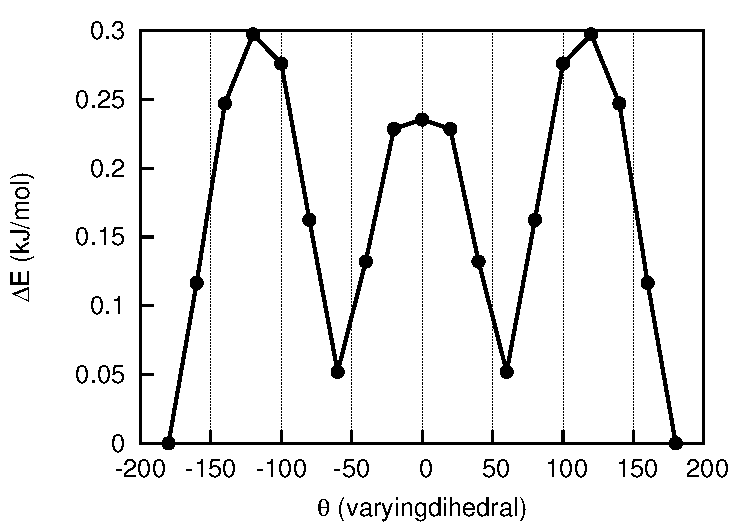
\includegraphics[width=8cm]{tolueno_sin_corr.pdf}
 \caption{Gráfico con la energía sin corregir vs rotación del ángulo dihiedro.}
\end{center}
\end{figure}

\begin{figure}[H]
 \begin{center}
 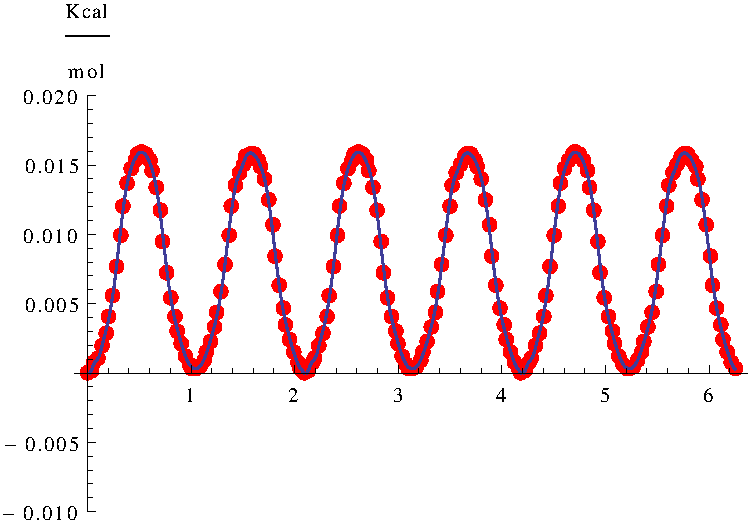
\includegraphics[width=8cm]{12345.pdf}
 \caption{Gráfico con la energía corregida vs rotación del ángulo dihiedro.}
\end{center}
\end{figure}

En la figura 2 se puede observar que, la energía no presenta el comportamiento esperado (seno ó coseno) esto es debido a que al realizar los cálculos de aproximación para obtener la energía para cada diferente conformación de la estructura de la mólecula, esta aproximación no es del todo buena, por lo que al realizar el tratamiento de los datos obtenidos (figura 3) se observa una gran mejoría en estos, observandose un comportamiento de dunción seno al momento de hacer la representación gráfica (figura 3). 
\subsection{Cálculo de funcionales de la densidad en átomos aislados}

\begin{figure}[H]
 \begin{center}
  \includegraphics[width=7cm]{/home/sebastian/trabajos/viep/moleculas/preporte/atomos/c-sphRho.pdf}
\includegraphics[width=7cm]{/home/sebastian/trabajos/viep/moleculas/preporte/atomos/nRho.pdf}
\includegraphics[width=7cm]{/home/sebastian/trabajos/viep/moleculas/preporte/atomos/o-sphRho.pdf}
 \end{center}
\caption{Gráficas de la densidad electrónica $\rho$ para átomos aislados.}
\end{figure}

Cuando se comprara la densidad electrónica de los tres átomos se observa un comportamiento similar (figura 4). Al comparar estos gráficos con los de las posterior sección podemos observar un comportamiento similar cuando más nos acercamos al  núcleo.

\subsection{Cálculo de funcionales de la densidad para un conjunto prueba de moléculas para la búsqueda de propiedades universales de la densidad electrónica}
Una vez obtenidos los resultados del cálculo de la densidad electrónica de todas las diferentes combinaciones de tipos de enlace se graficaron con el programa GNUPLOT. Con lo cual se obtuvieron las siguientes gráficas.\\
\begin{figure}[H]
\begin{center}
\includegraphics[width=4cm]{/home/sebastian/trabajos/viep/moleculas/preporte/graficos-d/c=c/d-C=C.pdf}
\includegraphics[width=4cm]{/home/sebastian/trabajos/viep/moleculas/preporte/graficos-d/c-c/d-C-C.pdf}
\includegraphics[width=4cm]{/home/sebastian/trabajos/viep/moleculas/preporte/graficos-d/c-h/d-C-H.pdf}
\includegraphics[width=4cm]{/home/sebastian/trabajos/viep/moleculas/preporte/graficos-d/c-n/d-C-N.pdf}
\includegraphics[width=4cm]{/home/sebastian/trabajos/viep/moleculas/preporte/graficos-d/c=o/d-C=O.pdf}
\includegraphics[width=4cm]{/home/sebastian/trabajos/viep/moleculas/preporte/graficos-d/c-o/d-C-O.pdf}
\includegraphics[width=4cm]{/home/sebastian/trabajos/viep/moleculas/preporte/graficos-d/n-h/d-N-H.pdf}
\includegraphics[width=4cm]{/home/sebastian/trabajos/viep/moleculas/preporte/graficos-d/o-h/d-O-H.pdf}
\end{center}
\caption{Gráficas de la densidad electrónica $\rho$.}
\end{figure}

En la figura 5 se muestran los gráficos obtenidos por el programa GNUPLOT al integrar todos los datos obtenidos por el programa DTK sobre el s(r) en el correspondiente enlace estudiado.\\
Se puede observar en la figura 5 que en todos los casos, la densidad electrónica se comporta de la misma manera mientas ás nos acercamos al 0, por lo que se podría creer que sigue un comportamiento igual para todos los casos.\\

\begin{figure}[H]
\begin{center}
\includegraphics[width=5cm]{/home/sebastian/trabajos/viep/moleculas/preporte/graficos-s/c=c/s-C=C.pdf}
\includegraphics[width=5cm]{/home/sebastian/trabajos/viep/moleculas/preporte/graficos-s/c-c/s-C-C.pdf}
\includegraphics[width=5cm]{/home/sebastian/trabajos/viep/moleculas/preporte/graficos-s/c-h/s-C-H.pdf}
\includegraphics[width=5cm]{/home/sebastian/trabajos/viep/moleculas/preporte/graficos-s/c-n/s-C-N.pdf}
\includegraphics[width=5cm]{/home/sebastian/trabajos/viep/moleculas/preporte/graficos-s/c=o/s-C=O.pdf}
\includegraphics[width=5cm]{/home/sebastian/trabajos/viep/moleculas/preporte/graficos-s/c-o/s-C-O.pdf}
\includegraphics[width=5cm]{/home/sebastian/trabajos/viep/moleculas/preporte/graficos-s/n-h/s-N-H.pdf}
\includegraphics[width=5cm]{/home/sebastian/trabajos/viep/moleculas/preporte/graficos-s/o-h/s-O-H.pdf}
\end{center}
\caption{Gráficos del gradiente reducido de la densidad electrónica s(r).}
\end{figure}
Al igual que en el caso anterior se puede observar un comportamiento similar para todos los casos.\\
Se muestran los gráficos obtenidos del cálculo de $|\nabla\rho|$, los datos obtenidos se agruparon en un sólo gráfico dependiendo del enlace estudiado.\\

\begin{figure}[H]
\begin{center}
\includegraphics[width=5cm]{/home/sebastian/trabajos/viep/moleculas/preporte/graficos-g/c=c/g-C=C.pdf}
\includegraphics[width=5cm]{/home/sebastian/trabajos/viep/moleculas/preporte/graficos-g/c-c/g-C-C.pdf}
\includegraphics[width=5cm]{/home/sebastian/trabajos/viep/moleculas/preporte/graficos-g/c-h/g-C-H.pdf}
\includegraphics[width=5cm]{/home/sebastian/trabajos/viep/moleculas/preporte/graficos-g/c-n/g-C-N.pdf}
\includegraphics[width=5cm]{/home/sebastian/trabajos/viep/moleculas/preporte/graficos-g/c=o/g-C=O.pdf}
\includegraphics[width=5cm]{/home/sebastian/trabajos/viep/moleculas/preporte/graficos-g/c-o/g-C-O.pdf}
\includegraphics[width=5cm]{/home/sebastian/trabajos/viep/moleculas/preporte/graficos-g/n-h/g-N-H.pdf}
\includegraphics[width=5cm]{/home/sebastian/trabajos/viep/moleculas/preporte/graficos-g/o-h/g-O-H.pdf}
\end{center}
\caption{Gráficos de la magnitud del gradiente de la densidad electrónica $|\nabla\rho|$.}
\end{figure}
Al igual que en el caso de la densidad el comportamiento es muy similar para todos los gráficos observados.\\ 
En la figura 5, se observan los gráficos obtenidos por el programa GNUPLOT en el cual se agruparon todos los datos obtenidos de una sola gráfica, dependiendo del tipo de enlace estudiado.\\
\begin{figure}[H]
\begin{center}
\includegraphics[width=4cm]{/home/sebastian/trabajos/viep/moleculas/preporte/graficos-l/c=c/l-C=C.pdf}
\includegraphics[width=4cm]{/home/sebastian/trabajos/viep/moleculas/preporte/graficos-l/c-c/l-C-C.pdf}
\includegraphics[width=4cm]{/home/sebastian/trabajos/viep/moleculas/preporte/graficos-l/c-h/l-C-H.pdf}
\includegraphics[width=4cm]{/home/sebastian/trabajos/viep/moleculas/preporte/graficos-l/c-n/l-C-N.pdf}
\includegraphics[width=4cm]{/home/sebastian/trabajos/viep/moleculas/preporte/graficos-l/c=o/l-C=O.pdf}
\includegraphics[width=4cm]{/home/sebastian/trabajos/viep/moleculas/preporte/graficos-l/c-o/l-C-O.pdf}
\includegraphics[width=4cm]{/home/sebastian/trabajos/viep/moleculas/preporte/graficos-l/n-h/l-N-H.pdf}
\includegraphics[width=4cm]{/home/sebastian/trabajos/viep/moleculas/preporte/graficos-l/o-h/l-O-H.pdf}
\caption{Gráficos del laplaciano de la densidad electrónica $\nabla^2\rho(r)$.} 
\end{center}

\end{figure}

Como se observo en los gráficos pasados (figuras 5, 6 y 7) se observa un comportamiento similar para todos los casos estudiados, siadno aquí más notorio que el comportamiento es casi igual, ya que las gráficas se superponen de tal forma que no se pueden distinguir. \\

\subsection{Evaluación del tiempo de ejecución del programa AIMALL para calcular Fuerza de Feyman}

\begin{figure}[H]
 \begin{center}
  \includegraphics[width=10cm]{12.pdf}
  \caption{Gráfico de tiempo de computo para cada molécula (Fuerza de Feyman).}
 \end{center}

\end{figure}
  Los tiempos que tarda el programa AIMALL son variados, y estos dependen del numero de electrones presentes en la molécula evaluada.

  \vfill
\begin{center}
\underline{Dr. Juan Manuel Solano Altamirano}\\
Responsable del programa.
\end{center}




\end{document}          
